\documentclass[12pt,a4paper]{article}

\usepackage[a4paper,margin=1in]{geometry}
\usepackage[T1]{fontenc}
\usepackage[utf8]{inputenc}
\usepackage{lmodern}
\usepackage{graphicx}
\usepackage{hyperref}
\usepackage{enumitem}
\usepackage{booktabs}
\usepackage{longtable}
\usepackage{array}
\usepackage{float}
\usepackage{setspace}

\setstretch{1.08}
\setlist[itemize]{leftmargin=1.5em}
\setlist[enumerate]{leftmargin=1.5em}

\title{\textbf{Design Report}\\Panda Scooter Project}
\author{Panda Scooter Team}
\date{}

\begin{document}
\maketitle
\tableofcontents
\newpage

\section{Introduction}

This report explains the design of Panda Scooter, a shared scooter platform that supports riders, dispatchers, and administrators in a unified workflow.

The system was designed to address the operational complexity of shared scooter management. A complete ride service must coordinate user authentication, scooter discovery, unlocking and locking, billing, fault reporting, vehicle dispatch, and administrative maintenance. A single-role application is not sufficient for these tasks, so Panda Scooter is implemented as a multi-app system with three frontends, one backend service, and one shared database.

The system scope of this report is summarized below.

\begin{table}[H]
\centering
\begin{tabular}{p{0.24\linewidth} p{0.56\linewidth}}
\toprule
\textbf{Component} & \textbf{Scope description} \\
\midrule
Rider mobile app & Scooter discovery, unlocking, riding, billing, fault reporting, wallet access, and personal record viewing. \\
Dispatcher mobile app & Vehicle lookup, scooter unlock/lock support, operational record viewing, and scooter information lookup. \\
Administrator web app & Fleet monitoring, zone management, parking point management, no-parking zone management, pricing, packages, and dispatcher management. \\
Backend service & Unified REST API, role-based authentication, business rules, MQTT integration, and data processing. \\
Database & Persistent storage for users, scooters, orders, wallets, subscriptions, zones, parking resources, and reports. \\
\bottomrule
\end{tabular}
\caption{System scope of the Panda Scooter project.}
\end{table}

The remainder of this report is organized as follows. Section 2 gives an overall overview of the project. Section 3 describes the system architecture. Sections 4 to 6 present module, database, and interface design. Section 7 summarizes the non-functional design considerations, and Section 8 concludes the report.

\section{Overall Overview}

\subsection{Project Positioning}

Panda Scooter is a shared scooter management platform for a three-role operational workflow. It supports rider-facing ride activities, dispatcher-side scooter handling, and administrator-side fleet management in one integrated system. The design covers an end-to-end business flow.

\subsection{Users and Runtime Environments}

The system is used by three types of users in different runtime environments:

\begin{table}[H]
\centering
\begin{tabular}{p{0.18\linewidth} p{0.24\linewidth} p{0.16\linewidth} p{0.32\linewidth}}
\toprule
\textbf{Role} & \textbf{Client} & \textbf{Runtime} & \textbf{Main usage} \\
\midrule
Rider & Mobile app & uni-app & Scooter discovery, unlock and lock, wallet, bills, fault reporting, and ride records. \\
Dispatcher & Mobile app & uni-app & Vehicle lookup, dispatch operations, scooter information, and dispatch history. \\
Administrator & Web app & Browser & Dashboard monitoring, zones, parking points, packages, pricing, and dispatcher management. \\
\bottomrule
\end{tabular}
\caption{User roles and runtime environments.}
\end{table}

\subsection{Technology Profile}

The overall technology profile is summarized below:

\begin{table}[H]
\centering
\begin{tabular}{p{0.18\linewidth} p{0.72\linewidth}}
\toprule
\textbf{Layer} & \textbf{Technology set} \\
\midrule
Mobile frontend & uni-app \\
Web frontend & Vue 3, AMap JSAPI \\
Backend & Spring Boot 3.2.5, Java 17, MyBatis, MQTT, Redis, MinIO \\
Database & MySQL 8.0 \\
Documentation & SpringDoc/OpenAPI \\
\bottomrule
\end{tabular}
\caption{Technical profile of the Panda Scooter system.}
\end{table}

\subsection{Deployment Model and Constraints}

The deployment model separates the system into three client deployments, one backend service, one database, and several external integration services. The rider and dispatcher clients run as WeChat mini-programs, the administrator client runs in a browser, and all three communicate with the same Spring Boot backend through HTTP. The backend interacts with MySQL, MQTT, AMap, and MinIO according to the needs of each business flow.

\begin{table}[H]
\centering
\begin{tabular}{p{0.24\linewidth} p{0.60\linewidth}}
\toprule
\textbf{Constraint type} & \textbf{Main constraints} \\
\midrule
Functional constraints & Strict role isolation, map-based scooter and zone queries, and MQTT-based scooter command handling. \\
Non-functional constraints & A maintainable data model, independent frontend evolution, and a scope that remains manageable within the current project. \\
\bottomrule
\end{tabular}
\caption{Main design constraints of the project.}
\end{table}

These constraints drive the architecture and module organization described in the next section.

\begin{figure}[H]
  \centering
  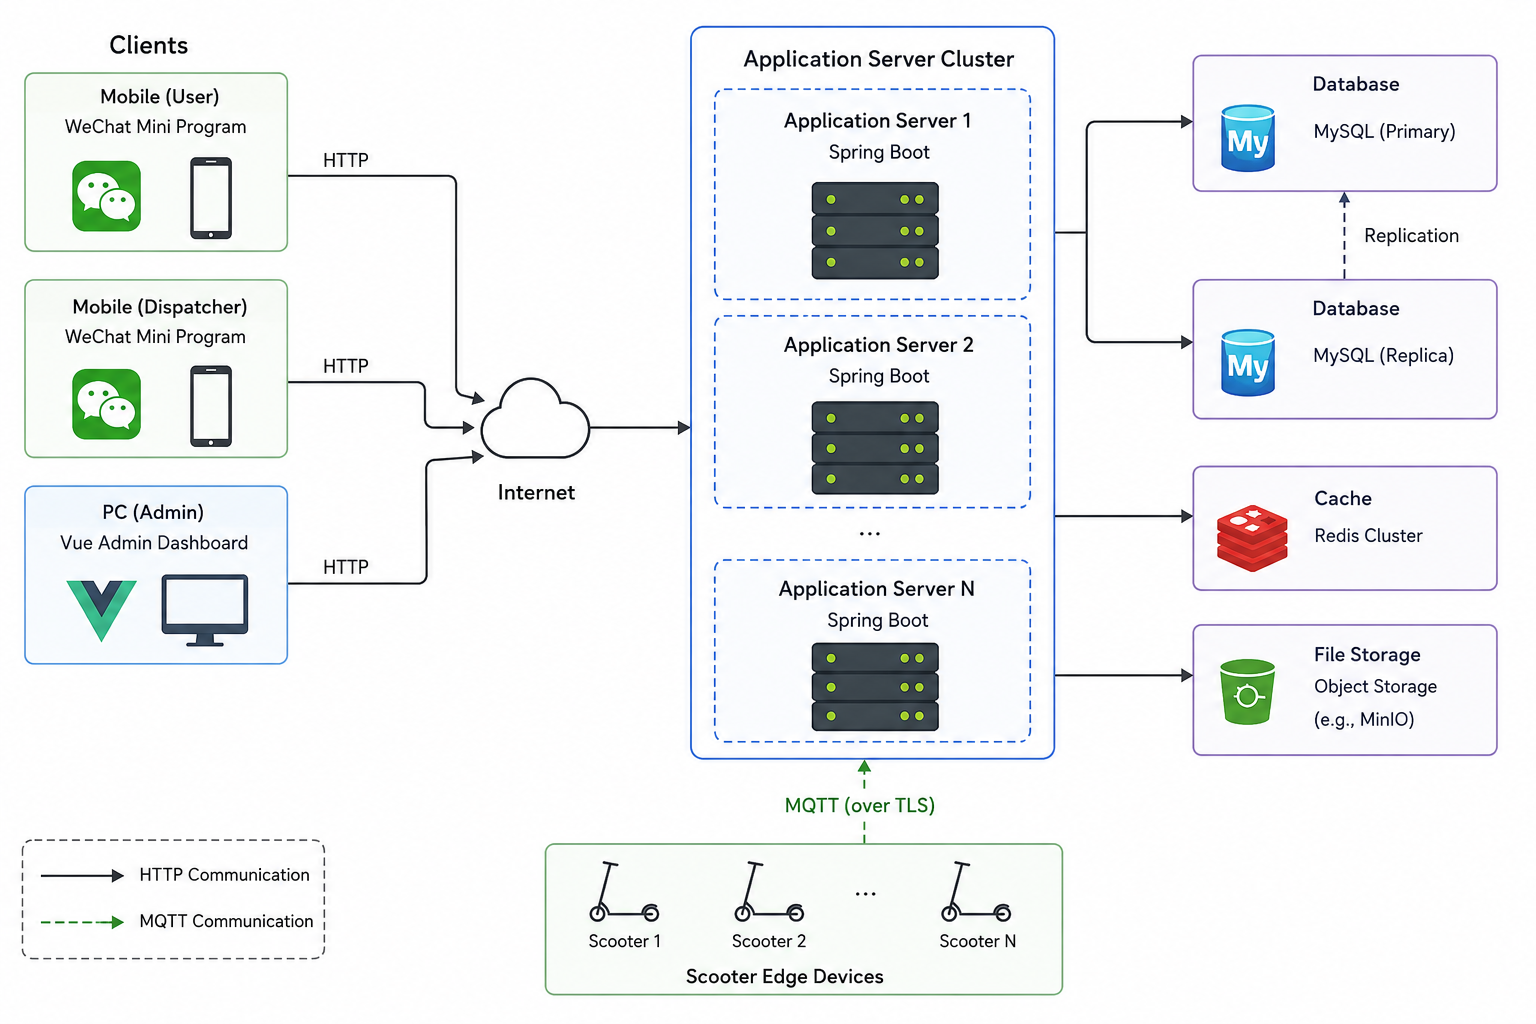
\includegraphics[width=\linewidth]{deployment_diagram.png}
  \caption{System deployment layout showing the rider mini-program, dispatcher mini-program, browser-based admin client, shared backend service, MySQL database, MQTT communication, AMap services, and MinIO storage.}
\end{figure}

\section{System Architecture Design}

\subsection{Architecture Overview}

The system follows a Browser-Server architecture. The rider and dispatcher applications are deployed as WeChat mini-programs, while the administrator interface runs in a browser-based web environment. This layout matches the project workflow: mobile users perform operational tasks on the move, and administrators manage fleet resources in a desktop-style control panel.

All client requests are routed to a shared Spring Boot backend, which acts as the central business hub of the system. The backend handles authentication, business processing, persistence access, and external service integration, so the frontends can remain lightweight and role-focused.

\begin{figure}[H]
  \centering
  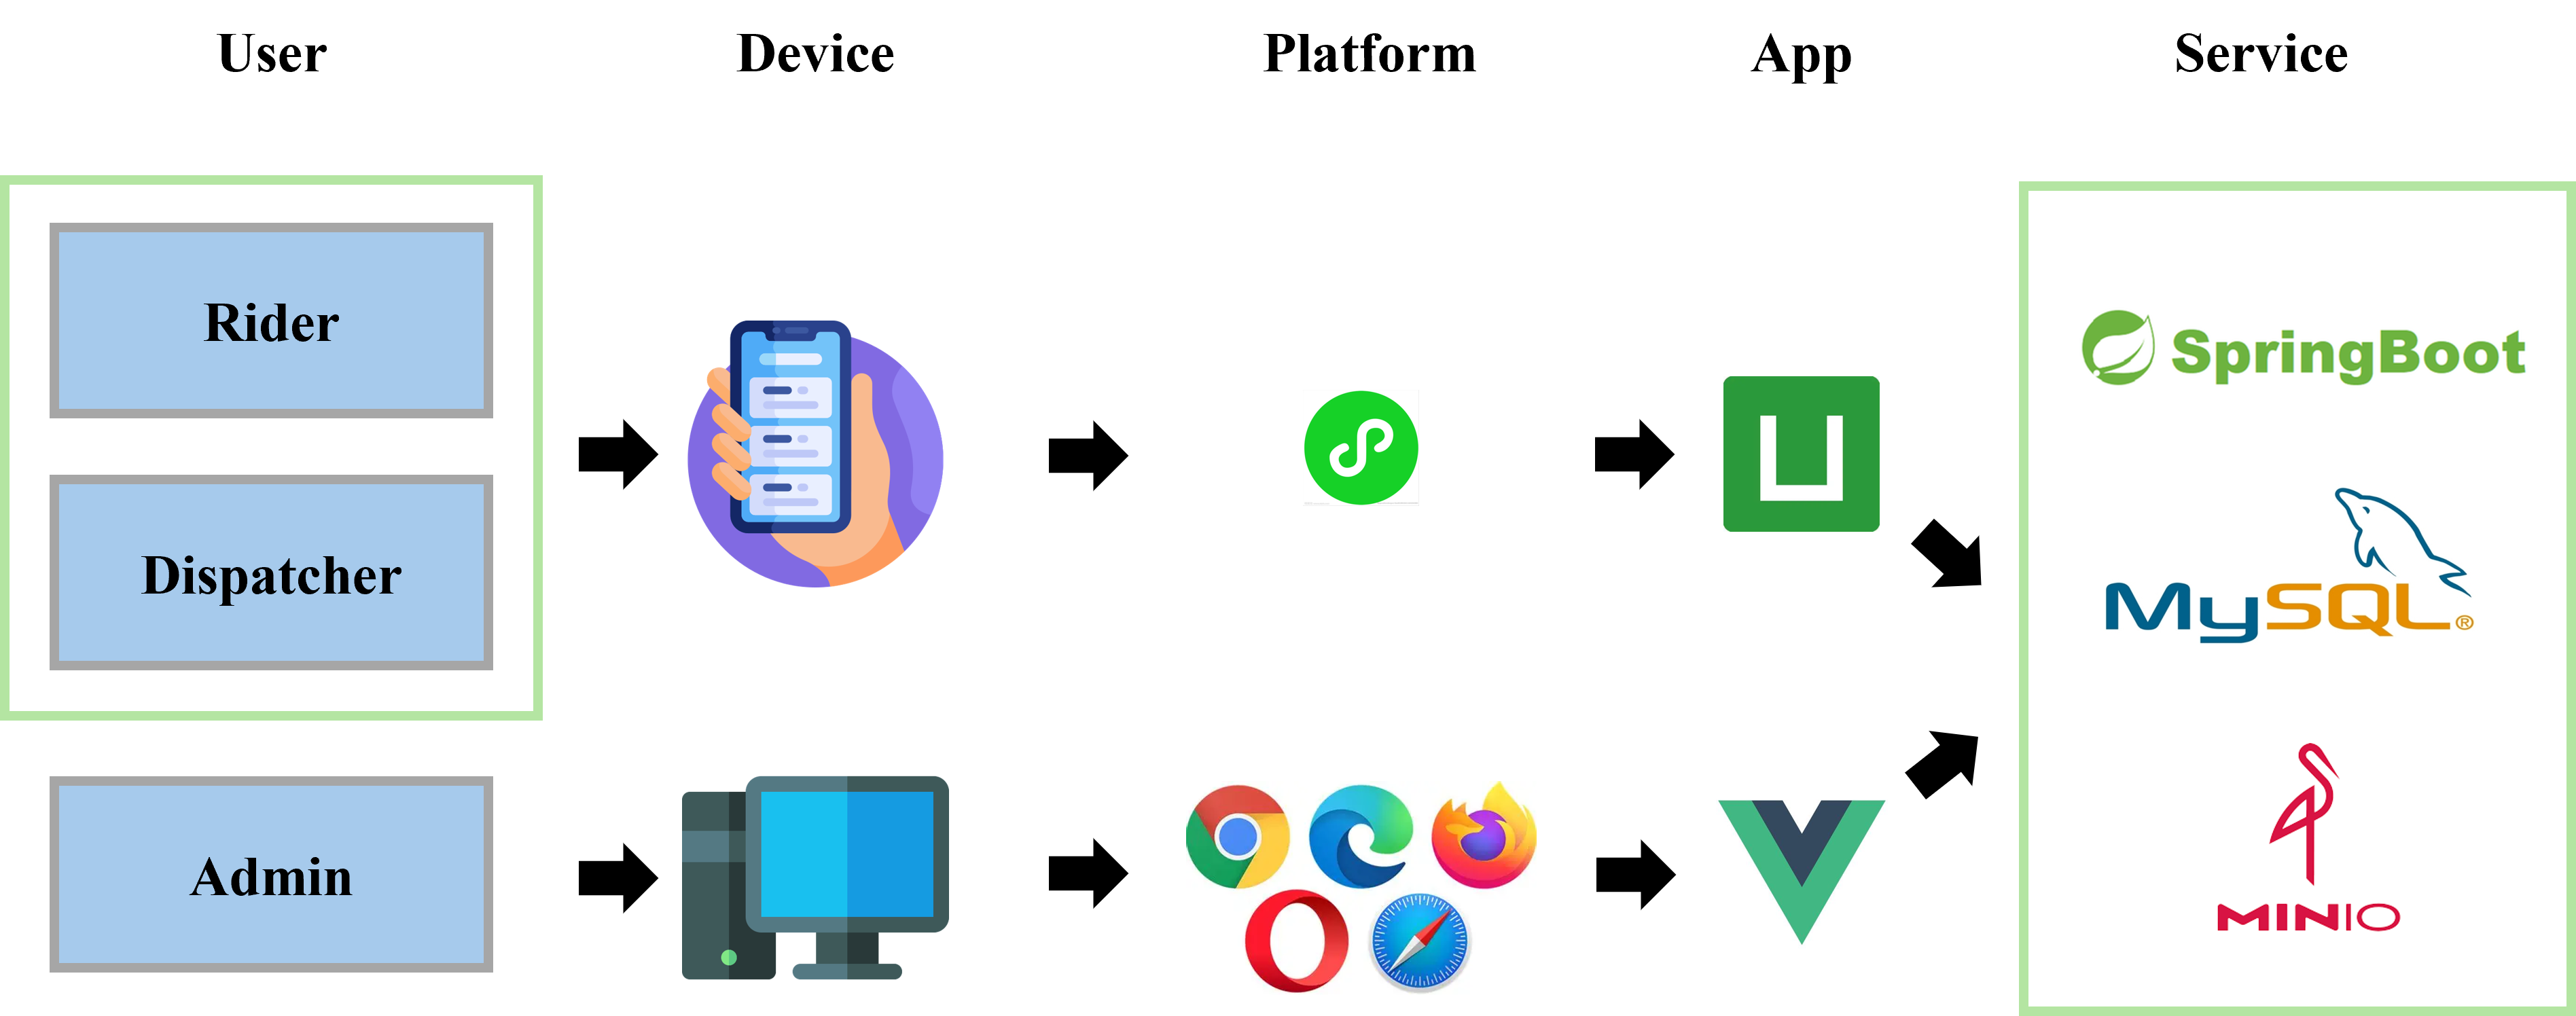
\includegraphics[width=\linewidth]{system_architacture.png}
  \caption{System architecture overview showing the rider mini-program, dispatcher mini-program, browser-based admin client, shared backend service, MySQL database, MQTT communication, AMap services, and MinIO storage.}
\end{figure}

\subsection{Client Layer Design}

The client layer consists of three role-specific applications, each designed for a different operational context.

\begin{table}[H]
\centering
\begin{tabular}{p{0.18\linewidth} p{0.70\linewidth}}
\toprule
\textbf{Client} & \textbf{Responsibility} \\
\midrule
Rider mini-program & Scooter discovery, unlocking, riding, billing, and fault reporting. \\
Dispatcher mini-program & Scooter lookup, dispatch actions, scooter status checks, and dispatch history review. \\
Admin browser client & Dashboard monitoring and the management of zones, parking points, scooters, packages, pricing rules, and dispatcher accounts. \\
\bottomrule
\end{tabular}
\caption{Responsibilities of the client layer.}
\end{table}

The separation of clients reduces interface clutter and keeps each front end aligned with the responsibilities of its target users. It also allows the mobile and browser clients to evolve independently without affecting the shared backend contract.

\subsection{Backend Service Design}

The backend is implemented as a Spring Boot service and is organized into three Maven modules:

\begin{table}[H]
\centering
\begin{tabular}{p{0.20\linewidth} p{0.66\linewidth}}
\toprule
\textbf{Module} & \textbf{Role in the backend} \\
\midrule
\texttt{panda-common} & Shared constants, JWT utilities, exception classes, base context, and response wrappers. \\
\texttt{panda-pojo} & Entities, DTOs, and VOs that describe the system data contracts. \\
\texttt{panda-server} & Executable application with controllers, services, interceptors, configuration, and MQTT logic. \\
\bottomrule
\end{tabular}
\caption{Backend module responsibilities.}
\end{table}

This structure separates reusable support code, data definitions, and runtime business logic. Controllers receive requests from the clients, services apply the business rules, and mappers transfer data between the application and the database. The backend therefore acts as the single coordination point for the entire platform.

\subsection{Data and Integration Layer Design}

The data and integration layer provides the persistent and external services required by the platform.

\begin{table}[H]
\centering
\begin{tabular}{p{0.18\linewidth} p{0.24\linewidth} p{0.48\linewidth}}
\toprule
\textbf{Service} & \textbf{Type} & \textbf{Role in the system} \\
\midrule
MySQL & Database & Stores users, scooters, orders, wallet records, subscriptions, zones, parking points, and fault reports. \\
MQTT & Messaging layer & Delivers scooter commands and supports telemetry exchange. \\
AMap & Map service & Supports map display and location-based scooter or zone queries. \\
MinIO & File storage & Stores uploaded files, especially fault-report images. \\
\bottomrule
\end{tabular}
\caption{Data and integration services.}
\end{table}

These services support the core business flow without forcing the frontend clients to manage low-level persistence or device communication directly. They also make the architecture easier to extend because each integration point is isolated in a dedicated service.

\subsection{Security and Access Isolation}

Security is enforced through role-based route separation and JWT-based interception. In \texttt{WebMvcConfiguration}, requests to \texttt{/user/**} are processed by the rider interceptor, requests to \texttt{/dispatcher/**} are processed by the dispatcher interceptor, and requests to \texttt{/admin/**} are processed by the admin interceptor.

Public routes such as login and verification are excluded from token checks so that authentication can complete before authorization is applied. This design keeps the security boundary clear while still allowing the user-facing login flow to remain accessible.

The architecture therefore combines role isolation, centralised backend control, and separated client responsibilities, which fits the shared-scooter workflow represented in the architecture diagram.

\section{Module Design}

The source code reveals a clear functional separation between rider, dispatcher, and admin modules. In addition, ride processing, billing, and MQTT communication are implemented as reusable backend services. Table~\ref{tab:module-overview} gives a concise module overview before the detailed description of each module.

\begin{table}[H]
\centering
\begin{tabular}{p{0.18\linewidth} p{0.28\linewidth} p{0.42\linewidth}}
\toprule
\textbf{Module} & \textbf{Primary focus} & \textbf{Typical outputs} \\
\midrule
Rider module & Ride lifecycle and personal service functions & Scooter discovery, unlock/lock, wallet, bills, faults, subscriptions, and ride records. \\
Dispatcher module & Operational scooter handling & Scooter lookup, dispatch actions, scooter information, and dispatch history. \\
Admin module & Platform maintenance and monitoring & Dashboard data, fleet management, zones, parking points, packages, pricing, and dispatcher administration. \\
Shared backend services & Cross-module business support & Ride processing, billing, and MQTT-based device communication. \\
\bottomrule
\end{tabular}
\caption{Overview of the major modules in the system.}
\label{tab:module-overview}
\end{table}

\subsection{Rider Module}

The rider module is the user-facing entry point for the ride workflow. It focuses on the complete rider journey from account access to ride settlement.

\begin{table}[H]
\centering
\begin{tabular}{p{0.24\linewidth} p{0.32\linewidth} p{0.34\linewidth}}
\toprule
\textbf{Function area} & \textbf{Main pages} & \textbf{Key behavior} \\
\midrule
Account management & \texttt{login}, \texttt{resetPassword}, \texttt{profile}, \texttt{account} & Registration, login, logout, deletion, password reset, and verification. \\
Ride discovery & \texttt{index}, \texttt{parking}, \texttt{unlock} & Map-based scooter discovery, parking point browsing, and unlock initiation. \\
Ride execution & \texttt{riding}, \texttt{unlock}, \texttt{lock} & Active ride display, ride termination, and order closure. \\
Finance and history & \texttt{wallet}, \texttt{bill}, \texttt{history} & Wallet balance, bill records, and ride history. \\
Fault and package support & \texttt{faults}, \texttt{reportFault} & Fault browsing, fault submission, and image upload. \\
\bottomrule
\end{tabular}
\caption{Rider module structure.}
\end{table}

The rider module is centered on the operational sequence of finding a scooter, starting a ride, ending the ride, and reviewing the settlement result. It also includes supporting functions such as fault reporting and subscription browsing.

\begin{figure}[H]
  \centering
  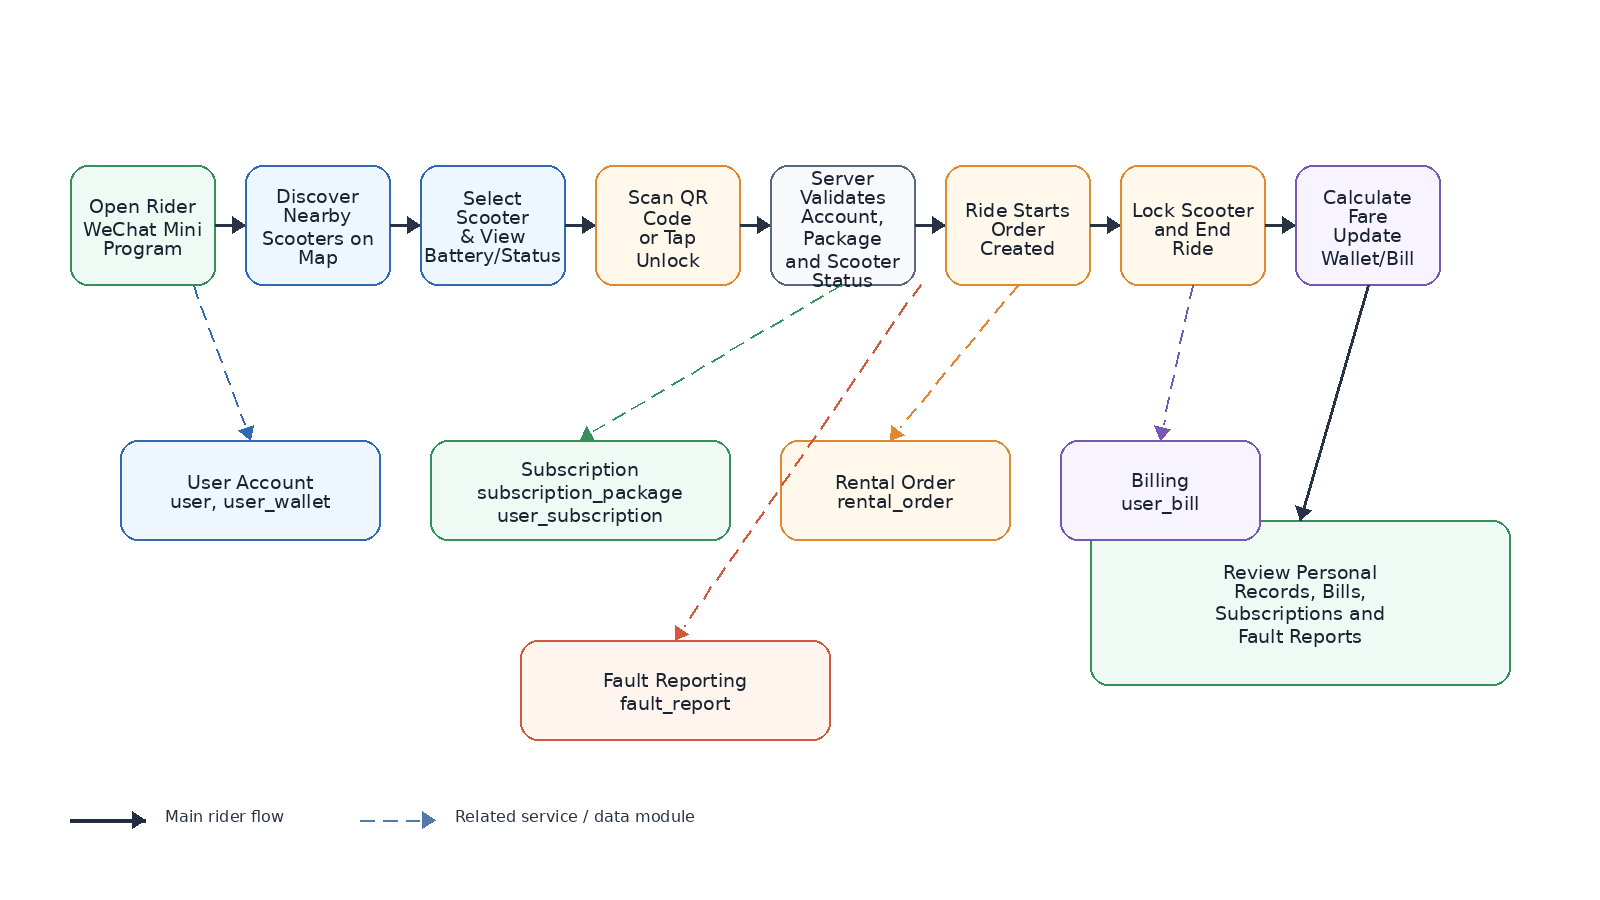
\includegraphics[width=\linewidth]{rider_module_flow.png}
  \caption{Rider module flow from scooter discovery to unlock, riding, lock, billing, and personal record review.}
\end{figure}

\subsection{Dispatcher Module}

The dispatcher module supports the operational staff who manage scooters in the field. Compared with the rider module, it is narrower in scope but more focused on vehicle handling and status checking.

\begin{table}[H]
\centering
\begin{tabular}{p{0.24\linewidth} p{0.32\linewidth} p{0.34\linewidth}}
\toprule
\textbf{Function area} & \textbf{Main pages} & \textbf{Key behavior} \\
\midrule
Account management & \texttt{login}, \texttt{resetPassword}, \texttt{profile}, \texttt{account} & Registration, login, logout, deletion, verification, and password reset. \\
Operational lookup & \texttt{index}, \texttt{vehicleLookup}, \texttt{scooterInfo} & Map inspection, scooter lookup by code, and scooter information viewing. \\
Field operations & \texttt{unlock}, \texttt{lock} & Operational scooter unlock and lock actions. \\
Record tracing & \texttt{history} & Dispatch history and traceability of operations. \\
\bottomrule
\end{tabular}
\caption{Dispatcher module structure.}
\end{table}

The dispatcher module is designed to make scooter handling quick and traceable. Its interface is smaller than the rider module, but each page is tied directly to a field operation.

\begin{figure}[H]
  \centering
  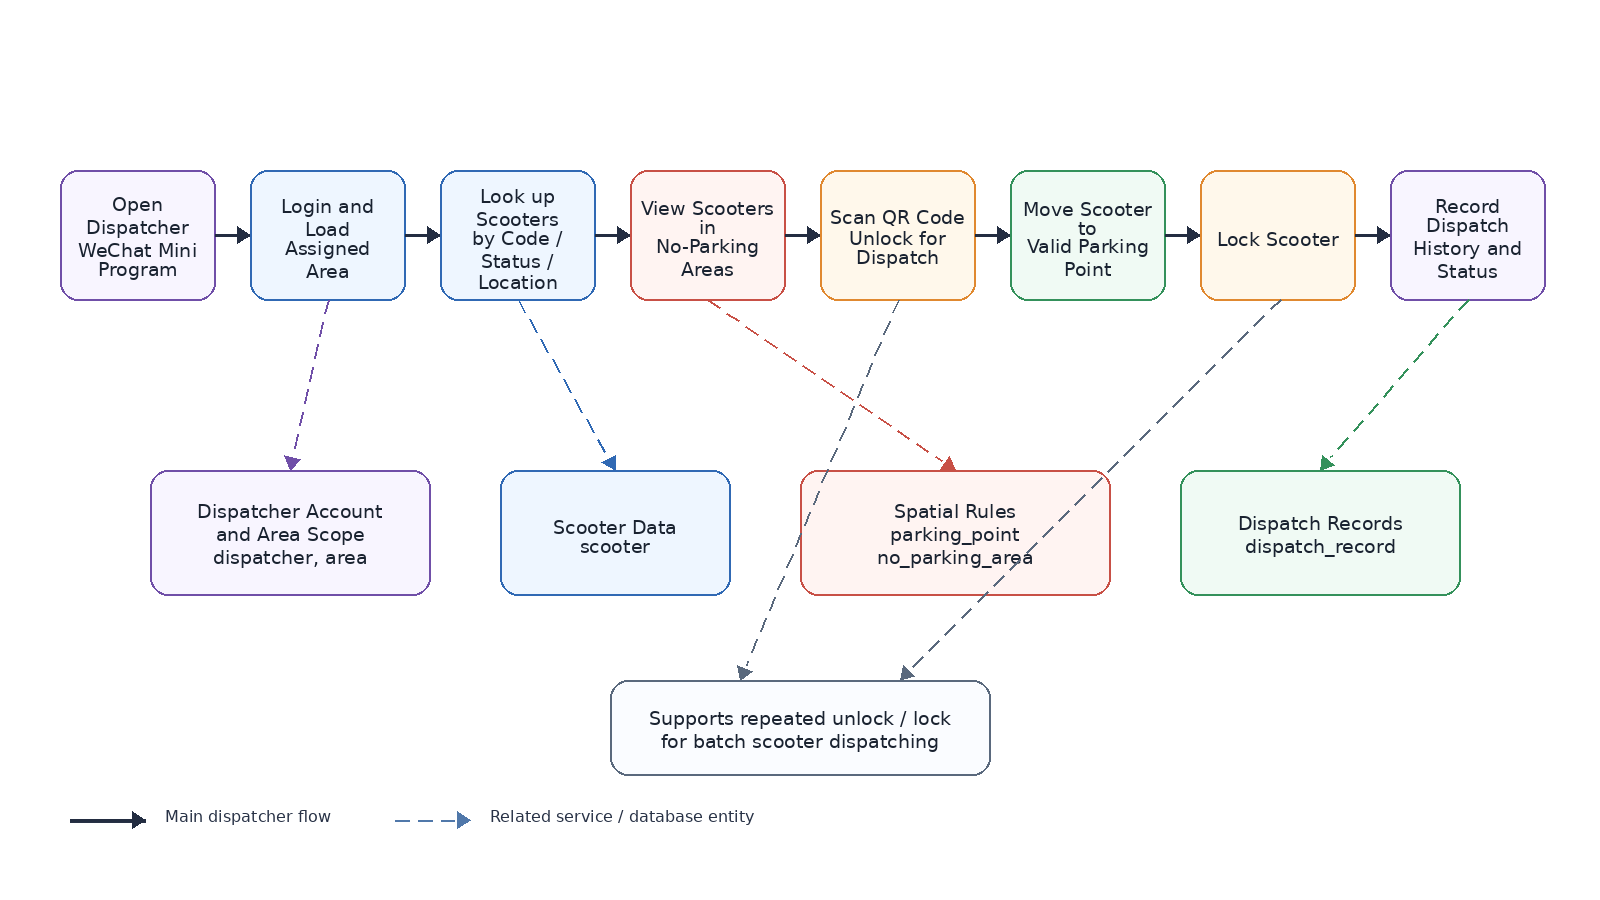
\includegraphics[width=\linewidth]{dispatcher_module_flow.png}
  \caption{Dispatcher module flow from scooter lookup to unlock, lock, and dispatch record tracking.}
\end{figure}

\subsection{Admin Module}

The admin module is the platform maintenance center. It organizes the management functions around the resources that need to be configured and monitored.

\begin{table}[H]
\centering
\begin{tabular}{p{0.24\linewidth} p{0.32\linewidth} p{0.34\linewidth}}
\toprule
\textbf{Resource area} & \textbf{Main views} & \textbf{Key behavior} \\
\midrule
Monitoring & \texttt{DashboardView} & Dashboard overview and live data inspection. \\
Fleet management & \texttt{VehicleManagementView} & Scooter list management. \\
Spatial management & \texttt{ZonesView}, \texttt{ZoneEditorView}, \texttt{ZoneDetailView} & Zone creation, editing, detail viewing, and deletion. \\
Parking control & \texttt{ParkingPointsView}, \texttt{ParkingPointEditorView}, \texttt{NoParkingZonesView}, \texttt{NoParkingZoneEditorView} & Parking point and no-parking area management. \\
Commercial settings & \texttt{PricingView}, \texttt{PackagesView} & Pricing rule and subscription package management. \\
Staff administration & \texttt{DispatchersView}, \texttt{LoginView} & Dispatcher administration and admin login functions. \\
\bottomrule
\end{tabular}
\caption{Admin module structure.}
\end{table}

The admin module is organized by resource type rather than by user journey. This makes the management interface more systematic and easier to extend when new operational resources are introduced.

\subsection{Shared Backend Services}

The shared backend services are not tied to a single frontend. They support the business rules that are reused by all three modules.

\begin{table}[H]
\centering
\begin{tabular}{p{0.20\linewidth} p{0.28\linewidth} p{0.40\linewidth}}
\toprule
\textbf{Service} & \textbf{Main responsibility} & \textbf{Supported modules} \\
\midrule
Ride service & Scooter lookup, unlock, lock, map data retrieval, unpaid-order payment, and ride history & Rider and dispatcher modules \\
Billing service & Wallet deduction, bill generation, and package-related settlement & Rider module and admin reporting \\
MQTT service & Publisher, listener, retry, and online-status support for scooter communication & Rider and dispatcher operational commands \\
\bottomrule
\end{tabular}
\caption{Shared backend services used across the modules.}
\end{table}

The ride service contains the most important business rules of the platform, such as one active ride per user, no unlock with unpaid orders, and ride settlement after locking. The MQTT layer enables asynchronous command delivery and telemetry exchange.

\begin{figure}[H]
  \centering
  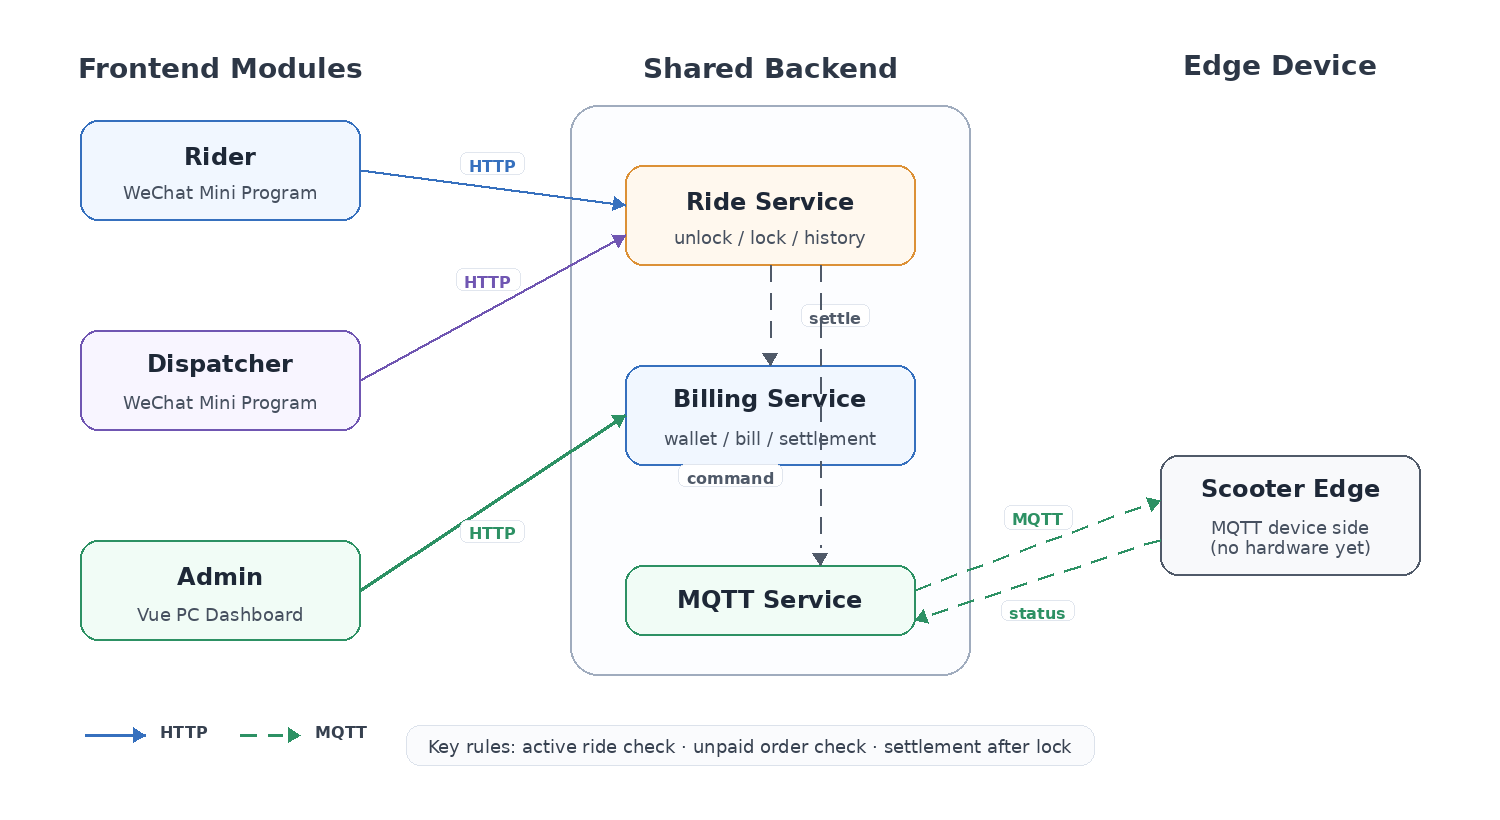
\includegraphics[width=\linewidth]{shared_backend_services_relationship_clean.png}
  \caption{Relationship diagram showing the rider, dispatcher, admin, ride service, billing service, and MQTT service connections.}
\end{figure}

\section{Database Design}

The database schema is defined in \texttt{docs/design report/bike\_system.sql}. The design is centered on the main business entities of the platform. The table structure is easy to map to the source code because most entities have direct Java counterparts in \texttt{panda-pojo}.

\subsection{Main tables}

\begin{longtable}{>{\raggedright\arraybackslash}p{0.22\linewidth}>{\raggedright\arraybackslash}p{0.25\linewidth}>{\raggedright\arraybackslash}p{0.43\linewidth}}
\toprule
\textbf{Table} & \textbf{Key fields} & \textbf{Purpose} \\
\midrule
\endhead
\texttt{admin} & \texttt{id}, \texttt{username}, \texttt{password}, \texttt{email}, \texttt{create\_time} & Administrator account information. \\
\texttt{user} & \texttt{id}, \texttt{username}, \texttt{password}, \texttt{email}, \texttt{create\_time} & Rider account information. \\
\texttt{dispatcher} & \texttt{id}, \texttt{name}, \texttt{password}, \texttt{email}, \texttt{area\_id}, \texttt{status} & Dispatcher identity and assigned area. \\
\texttt{scooter} & \texttt{id}, \texttt{code}, \texttt{battery}, \texttt{latitude}, \texttt{longitude}, \texttt{ride\_status}, \texttt{fault\_status} & Scooter status and location. \\
\texttt{rental\_order} & \texttt{user\_id}, \texttt{scooter\_id}, \texttt{start\_time}, \texttt{end\_time}, \texttt{total\_time}, \texttt{order\_status}, \texttt{pay\_status}, \texttt{amount} & Ride lifecycle and settlement. \\
\texttt{package\_order} & \texttt{user\_id}, \texttt{package\_id}, \texttt{price}, \texttt{order\_status}, \texttt{pay\_status} & Subscription package purchase orders. \\
\texttt{dispatch\_record} & \texttt{dispatcher\_id}, \texttt{scooter\_id}, \texttt{status}, \texttt{end\_time} & Dispatcher operations history. \\
\texttt{user\_wallet} & \texttt{user\_id}, \texttt{balance}, \texttt{update\_time} & User balance storage. \\
\texttt{user\_bill} & \texttt{user\_id}, \texttt{type}, \texttt{amount}, \texttt{balance\_after}, \texttt{order\_id}, \texttt{remark} & Wallet transaction ledger. \\
\texttt{subscription\_package} & \texttt{title}, \texttt{description}, \texttt{price}, \texttt{type} & Package catalog. \\
\texttt{user\_subscription} & \texttt{user\_id}, \texttt{package\_id}, \texttt{start\_time}, \texttt{end\_time}, \texttt{status} & Package ownership and validity. \\
\texttt{parking\_point} & \texttt{name}, \texttt{latitude}, \texttt{longitude}, \texttt{status} & Legal parking locations. \\
\texttt{no\_parking\_area} & \texttt{name}, \texttt{polygon}, \texttt{status} & Forbidden parking polygons. \\
\texttt{area} & \texttt{name}, \texttt{polygon}, \texttt{create\_time} & Operational area definition. \\
\texttt{pricing\_rule} & \texttt{price\_per\_min}, \texttt{base\_price}, \texttt{billing\_interval} & Ride pricing configuration. \\
\texttt{fault\_report} & \texttt{user\_id}, \texttt{scooter\_id}, \texttt{description}, \texttt{image\_url}, \texttt{status} & Fault reporting. \\
\bottomrule
\end{longtable}

\subsection{Relationship and indexing design}

The schema uses indexes on fields that are frequently queried in business flows, such as \texttt{user\_id}, \texttt{scooter\_id}, \texttt{dispatcher\_id}, and \texttt{order\_id}. This supports ride lookup, wallet reconciliation, dispatch record queries, and audit-like operations.

The \texttt{scooter} table stores both identity and runtime state, which makes map display and operational control straightforward. The \texttt{rental\_order} and \texttt{user\_bill} tables form the financial core of the system, while \texttt{user\_subscription} records time-bound package ownership.

\begin{figure}[H]
  \centering
  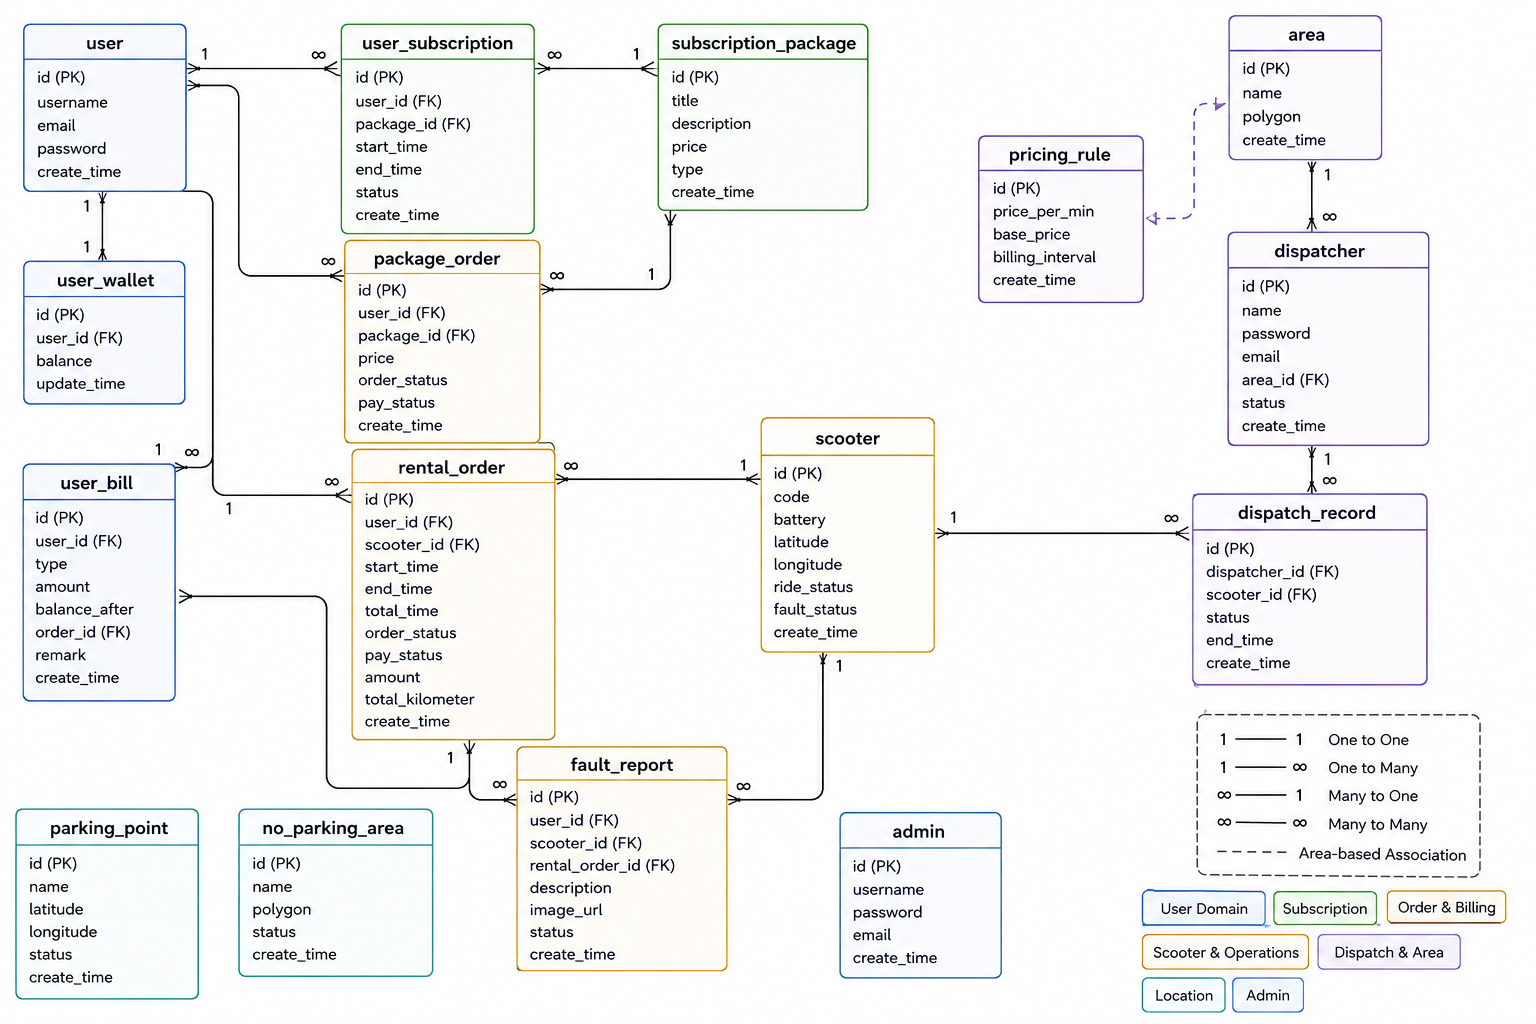
\includegraphics[width=\linewidth]{entity_relationship_diagram.png}
  \caption{ER diagram showing the relations among riders, dispatchers, scooters, orders, bills, subscriptions, zones, and parking resources.}
\end{figure}

\section{Interface Design}

The backend uses REST-style interfaces and a unified response wrapper, \texttt{Result<T>}, to keep response handling consistent across the frontends. The design also uses SpringDoc, which supports interface documentation and interactive API inspection.

\subsection{API inventory compiled from the documentation}

The following API list is compiled from the generated documentation files in \texttt{docs/design report}. Every documented endpoint is included in the report and grouped by role and function so that the interface structure is easy to trace. Some account-related routes are intentionally shared across rider and dispatcher clients because both frontends reuse the same login and verification flow.

\begin{table}[H]
\centering
\begin{tabular}{p{0.20\linewidth} p{0.18\linewidth} p{0.42\linewidth}}
\toprule
\textbf{Role} & \textbf{Endpoint count} & \textbf{Design focus} \\
\midrule
Rider & 19 & Account lifecycle, ride flow, wallet, bills, faults, and subscriptions. \\
Dispatcher & 12 & Shared account flow, dispatch operations, map queries, and scooter status lookup. \\
Administrator & 28 & Monitoring, pricing, package, zone, no-parking, dispatcher, parking point, and fleet management. \\
\bottomrule
\end{tabular}
\caption{Coverage summary of the documented APIs.}
\end{table}

\subsubsection{Rider API inventory}

\begin{longtable}{p{0.22\linewidth} p{0.56\linewidth} p{0.14\linewidth}}
\toprule
\textbf{Function group} & \textbf{Documented endpoints} & \textbf{Purpose} \\
\midrule
\endhead
Account lifecycle & \texttt{POST /user/signin}, \texttt{POST /user/login}, \texttt{POST /user/logout}, \texttt{DELETE /user/delete}, \texttt{GET /user/verification}, \texttt{POST /user/password} & Rider registration, login, logout, deletion, verification, and password reset. \\
Wallet and bills & \texttt{POST /user/bill}, \texttt{GET /user/bills}, \texttt{GET /user/wallet} & Wallet charge and consumption records, bill history, and wallet balance. \\
Ride and map & \texttt{GET /ride-history}, \texttt{POST /unpaid-order}, \texttt{GET /user/info}, \texttt{GET /map}, \texttt{GET /scooter}, \texttt{POST /scooter/unlock}, \texttt{POST /scooter/lock} & Ride lookup, scooter discovery, map query, unlock/lock, unpaid-order payment, and ride information. \\
Fault and subscription & \texttt{GET /faults}, \texttt{POST /fault}, \texttt{GET /subscription} & Fault report browsing, fault submission, and subscription package browsing. \\
\bottomrule
\end{longtable}

\begin{itemize}
  \item The rider API set supports the full lifecycle from account creation to trip completion.
  \item The wallet and bill endpoints form the financial trail used by the ride settlement flow.
  \item The fault and subscription routes extend the rider experience beyond the core riding scenario.
\end{itemize}

\subsubsection{Dispatcher API inventory}

\begin{longtable}{p{0.22\linewidth} p{0.56\linewidth} p{0.14\linewidth}}
\toprule
\textbf{Function group} & \textbf{Documented endpoints} & \textbf{Purpose} \\
\midrule
\endhead
Account lifecycle & \texttt{POST /user/signin}, \texttt{POST /user/login}, \texttt{POST /user/logout}, \texttt{DELETE /user/delete}, \texttt{GET /user/verification}, \texttt{POST /user/password} & Dispatcher registration, login, logout, deletion, verification, and password reset. \\
Operational information & \texttt{GET /user/info}, \texttt{GET /user/dispatch-history} & Dispatcher profile information and dispatch history. \\
Map and scooter operations & \texttt{GET /map}, \texttt{POST /scooter/unlock}, \texttt{POST /scooter/lock}, \texttt{GET /scooter/info} & Map query, scooter unlock/lock, and scooter information lookup. \\
\bottomrule
\end{longtable}

\begin{itemize}
  \item Dispatcher endpoints reuse the same authentication model as riders, which keeps the account workflow consistent across mobile clients.
  \item Operational APIs are concentrated around map inspection and scooter command execution.
\end{itemize}

\subsubsection{Admin API inventory}

\begin{longtable}{p{0.22\linewidth} p{0.56\linewidth} p{0.14\linewidth}}
\toprule
\textbf{Function group} & \textbf{Documented endpoints} & \textbf{Purpose} \\
\midrule
\endhead
Authentication & \texttt{POST /admin/login}, \texttt{POST /admin/logout} & Admin login and logout. \\
Monitoring & \texttt{GET /admin/overview}, \texttt{GET /admin/live-data} & Dashboard metrics and real-time data. \\
Pricing & \texttt{GET /admin/pricing-rules}, \texttt{PUT /admin/pricing-rules} & Pricing rule retrieval and updates. \\
Packages & \texttt{GET /admin/packages}, \texttt{POST /admin/packages}, \texttt{PUT /admin/packages/\{id\}}, \texttt{DELETE /admin/packages/\{id\}} & Subscription package management. \\
Zones & \texttt{GET /admin/zones}, \texttt{POST /admin/zones}, \texttt{GET /admin/zones/\{id\}}, \texttt{PUT /admin/zones/\{id\}}, \texttt{DELETE /admin/zones/\{id\}} & Operational zone management. \\
No-parking zones & \texttt{GET /admin/no-parking-zones}, \texttt{POST /admin/no-parking-zones}, \texttt{PUT /admin/no-parking-zones/\{id\}}, \texttt{DELETE /admin/no-parking-zones/\{id\}} & No-parking polygon management. \\
Dispatchers & \texttt{GET /admin/dispatchers}, \texttt{POST /admin/dispatchers}, \texttt{PUT /admin/dispatchers/\{id\}}, \texttt{DELETE /admin/dispatchers/\{id\}} & Dispatcher account management. \\
Parking points & \texttt{GET /admin/parking-points}, \texttt{POST /admin/parking-points}, \texttt{PUT /admin/parking-points/\{id\}}, \texttt{DELETE /admin/parking-points/\{id\}} & Parking point management. \\
Scooters & \texttt{GET /admin/scooters} & Fleet list query. \\
\bottomrule
\end{longtable}

\begin{itemize}
  \item The admin API set is the largest group because it combines monitoring and maintenance functions.
  \item Management endpoints are arranged by resource type so the dashboard can mirror the operational structure of the system.
\end{itemize}

\subsection{Authorization}

The platform uses JWT-based authorization to separate the three roles and protect their private routes. After successful login, the backend issues a token that is carried by the client in subsequent requests. The token is stored in the client and attached to protected requests so that the backend can identify the current role and enforce access control.

The token payload includes the core identity claims needed by the backend, such as the user identifier, username or name, role information, and token timing information. In practice, the payload is encoded into a compact JWT structure, which is then transmitted as a bearer token. The backend decodes the token, verifies its signature, and extracts the claims before the request is allowed to reach the business layer.

\begin{table}[H]
\centering
\begin{tabular}{p{0.24\linewidth} p{0.60\linewidth}}
\toprule
\textbf{JWT claim} & \textbf{Meaning} \\
\midrule
\texttt{id} & Unique identifier of the authenticated account. \\
\texttt{username} or \texttt{name} & Display identity of the current account. \\
\texttt{role} & Role label used for access control, such as rider, dispatcher, or administrator. \\
\texttt{iat} & Issued-at timestamp used by the token library. \\
\texttt{exp} & Expiration timestamp used to limit token lifetime. \\
\bottomrule
\end{tabular}
\caption{Typical information carried in the JWT payload.}
\end{table}

The protected namespaces are \texttt{/user/**}, \texttt{/dispatcher/**}, and \texttt{/admin/**}. Public routes such as login and verification remain open so that the token can be obtained before authorization is applied.

\subsection{Response format}

The backend returns a unified \texttt{Result<T>} wrapper for all interfaces. This design keeps the client-side handling logic simple because the frontends only need to check one response structure regardless of the business function being called.

\begin{table}[H]
\centering
\begin{tabular}{p{0.30\linewidth} p{0.58\linewidth}}
\toprule
\textbf{Response field} & \textbf{Meaning} \\
\midrule
\texttt{code} & Status code used by the frontend to judge whether the request succeeded. \\
\texttt{msg} & Human-readable message returned by the backend. \\
\texttt{data} & Business payload returned to the client. \\
\bottomrule
\end{tabular}
\caption{Common response wrapper structure.}
\end{table}

\begin{table}[H]
\centering
\begin{tabular}{p{0.26\linewidth} p{0.60\linewidth}}
\toprule
\textbf{Response type} & \textbf{Typical role in the system} \\
\midrule
Success response & Carries the correct code '0' and the requested business data. \\
Failure response & Carries the error code '1' and message used to explain why the request failed. \\
\bottomrule
\end{tabular}
\caption{Response behavior in the unified wrapper.}
\end{table}

\section{Non-functional Design}

The non-functional design covers security, performance, maintainability, and reliability.

\subsection{Security design}

Security is implemented through role-based JWT interceptors and route separation. Each role has its own protected namespace, which reduces the risk of cross-role access. CORS configuration is also defined globally so that the frontend applications can communicate with the backend during development and deployment.

Password handling is implemented through server-side processing before storage. Validation is used to reduce malformed requests, and the global exception handling strategy keeps error responses predictable.

\subsection{Performance design}

The design uses index-supported relational tables and bounded map queries. The scooter map data is filtered by the current map center and scale, which avoids returning an unnecessary full-data set. The admin data overview and live data endpoints are also query-driven so that the dashboard can refresh metrics without heavy client-side processing.

MQTT is used for asynchronous scooter communication instead of forcing all device operations through synchronous HTTP calls. This helps reduce pressure on the main request path and better matches the device-control scenario.

\subsection{Maintainability design}

The multi-module backend structure separates common utilities, data objects, and runnable business services. The frontends are also separated by role, so the rider app, dispatcher app, and admin dashboard can evolve independently. The use of MyBatis mappers and explicit DTO/VO classes makes the code easier to trace from request to persistence.

\subsection{Reliability design}

The system uses unified result wrapping and global exception handling, which makes failures easier to interpret on the client side. The ride flow is stateful and guarded by business checks such as one active ride per user and unpaid-order blocking. MQTT retry and online-status support further improve operational reliability for scooter commands.

\subsection{Known limitations}

The current implementation is still a course project, so some aspects are simplified:
\begin{itemize}
  \item scooter hardware communication is simulated rather than deployed on full-scale devices;
  \item map display and zone calculations rely on the configured map service and current data format;
  \item some admin analytics are produced through direct queries rather than a dedicated reporting subsystem;
  \item the UI design is functional but not yet standardized as a complete design system.
\end{itemize}

\begin{table}[H]
\centering
\begin{tabular}{p{0.20\linewidth} p{0.32\linewidth} p{0.36\linewidth}}
\toprule
\textbf{Aspect} & \textbf{Design choice} & \textbf{Effect} \\
\midrule
Security & JWT interceptors and role-specific paths & Reduces unauthorized access across user roles. \\
Performance & Indexed relational tables and map-scale filtering & Keeps requests bounded and predictable. \\
Maintainability & Multi-module backend and DTO/VO structure & Makes the codebase easier to trace and extend. \\
Reliability & Global exception handling and MQTT retry support & Improves failure visibility and command delivery. \\
\bottomrule
\end{tabular}
\caption{Summary of non-functional design decisions.}
\end{table}

\section{Summary}

Panda Scooter demonstrates a complete end-to-end shared scooter workflow that covers rider operations, dispatcher operations, and administrative management. The system combines a layered architecture, role-separated frontends, a shared Spring Boot backend, and a relational database schema that maps directly to the major business entities in the platform.

From a design perspective, the project shows that the three user roles can be supported in a consistent and maintainable way. The modular backend structure, the unified API response pattern, and the clear separation between business services and integration services all help reduce coupling and make the system easier to extend.

The current implementation is already able to support the main business flow of a scooter-sharing platform, but there is still room for improvement in areas such as analytics, device integration, automated testing, UI consistency, and scalability. These directions define the next stage of development if the project is continued beyond the current course scope.

\end{document}
